\documentclass[10pt,twocolumn,twoside]{IEEEtran}

\usepackage{afterpage}
\usepackage{bold-extra}
\usepackage{color}
\usepackage{float}
\usepackage{graphicx}
\usepackage{listings}
\usepackage{subfigure}

%%%%%%%%%%%%%%%
%%% Colours %%%
%%%%%%%%%%%%%%%

\definecolor{darkgreen}{rgb}{0, 0.6, 0}
\definecolor{lightgrey}{gray}{0.9}

%%%%%%%%%%%
% Figures %
%%%%%%%%%%%

% Define shorter ways to include individual images
\newcommand{\stufig}[4]						% images with default placement
{
	\begin{figure}
	\begin{center}
		\includegraphics[#1]{#2}
		\caption{#3}
		\label{#4}
	\end{center}
	\end{figure}
}

\newcommand{\stufigex}[5]					% images with specified placement
{
	\begin{figure}[#5]
	\begin{center}
		\includegraphics[#1]{#2}
		\caption{#3}
		\label{#4}
	\end{center}
	\end{figure}
}

\newcommand{\stufigexx}[5]				% full-width images with specified placement
{
	\begin{figure*}[#5]
	\begin{center}
		\includegraphics[#1]{#2}
		\caption{#3}
		\label{#4}
	\end{center}
	\end{figure*}
}

% Define the stusubfig environment
\newenvironment{stusubfig}[1]
{
	\begin{figure*}[#1]
	\begin{center}
}
{
	\end{center}
	\end{figure*}
}

%%%%%%%%%%%%%%%%%
% Code Listings %
%%%%%%%%%%%%%%%%%

% Create a new type of float (called a stulisting) for listings
\floatstyle{ruled}
\newfloat{stulisting}{thp}{lop}
\floatname{stulisting}{Listing}

% Setup before using the listings package
\renewcommand{\lstlistingname}{\textbf{Listing}}
\renewcommand{\thelstlisting}{\textbf{\arabic{lstlisting}}}

\lstdefinelanguage{Pseudocode}{
morekeywords={and,assert,break,case,continue,default,down,each,else,for,function,if,not,null,or,rangeswitch,ref,return,switch,then,this,throw,to,up,var,while},
sensitive=true,
morecomment=[l]{//},
morecomment=[s]{/*}{*/}
}

\lstdefinestyle{Default}{
abovecaptionskip=0.5cm,
basicstyle=\scriptsize\ttfamily,
belowcaptionskip=0.5cm,
belowskip=0.5cm,
columns=fixed,
%commentstyle=\color{darkgreen},
commentstyle=\textit, % changed from the thesis (green text looks unprofessional in a journal paper)
language=Pseudocode,
%numbers=left,
numbers=none, % changed from the thesis (line numbers are less relevant here)
numbersep=5pt,
numberstyle=\tiny,
mathescape=true,
showstringspaces=false,
stepnumber=1,
tabsize=4
}

\lstdefinestyle{Snippet}{
abovecaptionskip=0.5cm,
aboveskip=0.5cm,
basicstyle=\small\ttfamily,
belowcaptionskip=0.5cm,
belowskip=0.5cm,
columns=fixed,
commentstyle=\color{darkgreen},
frame=lines,
keywordstyle=\small\bfseries,
language=Pseudocode,
numbers=none,
mathescape=true,
showstringspaces=false,
stepnumber=1,
tabsize=4
}

% For C++ function prototypes
\lstdefinestyle{Prototype}{
abovecaptionskip=0.5cm,
basicstyle=\small\ttfamily,
belowcaptionskip=0.5cm,
belowskip=0.5cm,
columns=fixed,
commentstyle=\color{darkgreen},
language=C++,
numbers=none,
mathescape=true,
showstringspaces=false,
stepnumber=1,
tabsize=4
}

%%%%%%%%%%%%%%%%%
% Main Document %
%%%%%%%%%%%%%%%%%

\begin{document}

%\title{The Use of Zipping Algorithms to Facilitate Interaction with Image Partition Forests}
\title{Zipping Partition Forests to Edit Segmented Images}
%\title{Editing Segmented Images by Zipping Partition Forests}
%\title{Manipulating Segmented Images by Zipping Partition Forests}

\author{Stuart Golodetz, Irina Voiculescu and Stephen Cameron}

\date{\today}
\maketitle

\begin{abstract}
%\noindent The segmentation of medical scans and the subsequent identification of key features therein is an important precursor to many medical imaging applications. One interesting approach is to start by partitioning the image into a region hierarchy, in which each node represents a contiguous region of the image; however, once built, the hierarchy tends to be static, making the results very dependent on the initial tree construction process. In this paper, we describe our approach to the automatic feature identification problem, in particular explaining why modifying the hierarchy at a later stage can be useful, and how it can be achieved. (TODO: The focus of the paper has changed slightly -- update this to reflect that.)

\noindent The segmentation of images and the subsequent identification of key features therein are important components of applications in a variety of contexts, including those such as medical imaging where extremely high levels of accuracy are required. However, both remain challenging to completely automate, and so there is often a need for domain specialists to be able to edit the results produced by automatic tools; the editing methods used evidently depend strongly on how the results are represented. One helpful representation is the \emph{image partition forest} (IPF), or region hierarchy, a tree-like data structure in which each node represents a contiguous region of the image. Unfortunately, since little research attention has been devoted in the past to ways of interacting with IPFs, it can be difficult for domain specialists to make changes to them after they have been built -- this imposes much higher accuracy requirements on tools that produce them, since those with the expert knowledge needed to correct any mistakes made by the tools are actively prevented from doing so. In this paper, we therefore present a set of algorithms that can be used to facilitate interactive changes to IPFs. The algorithms were implemented as a core part of \emph{millipede}, a cross-platform tool for 3D segmentation, feature identification and visualisation, and we highlight in particular the way in which the user experience was improved as a result.
\end{abstract}

%#####################
\section{Introduction}
%#####################

%TODO \cite{gvccimi08,gvcispa09}

Image segmentation, the problem of how to partition an image into regions that have some meaning in a given domain, and feature identification, the problem of how to ascribe meaning to some or all of those regions, are important tasks in a variety of practical contexts \cite{?}. However, as observed in \cite{golodetz11}, both remain challenging to completely automate due to the difficulty of specifying what constitutes a meaningful region in a particular context. In certain domains, particularly those such as medical imaging where the consequences of incorrect or inaccurate segmentation can be significant, it is therefore extremely important for domain specialists (e.g.~radiologists in the case of medical images) to be able to interact with the results of a segmentation produced by an automated tool in order to correct any mistakes made.

Depending on the kind of segmentation used\footnotemark, these results can be represented in a variety of different ways and require varying different methods of interaction. For example, editing a segmentation result produced by thresholding (a technique that classifies individual pixels of the image as either background or foreground based on their value relative to a constant threshold, e.g.~all pixels $<= 128$ are background and all pixels $> 128$ are foreground) might involve changing the threshold value and re-segmenting the image, whereas editing a segmentation produced by a snakes approach (e.g.~\cite{kass88,lobregt95}) might involve a human user dragging the snake contour around using a graphical user interface.

\footnotetext{A survey of many of the different kinds of segmentation can be found in \cite{golodetz11}.}

One type of segmentation result that can provide a great deal of useful information for further processing is what we call the \emph{image partition forest} (IPF) representation\footnotemark, which represents an image as a hierarchy of partitions (the details of this representation will be described in \S\ref{sec:ipfs}). This representation is useful because it consists of related segmentations of the image at different scales, providing a helpful space in which to search for regions corresponding to image features of different sizes. An IPF can be produced as the result of a number of different segmentation approaches, and detailed techniques for constructing one using watershed/waterfall segmentation are described in \cite{golodetz11}.

\footnotetext{The same data structure has appeared elsewhere in the literature under a variety of other names, e.g.~hierarchy of (region adjacency) graphs \cite{kropatsch04,nacken95,shen97}, hierarchical attributed region adjacency graph \cite{fischer04}, hierarchy of partitions \cite{haxhimusa03,lezoray06}, picture tree \cite{andrade03}, graph pyramid \cite{kerren06}, bounded irregular pyramid \cite{marfil07} and segmentation graph \cite{borenstein06}.}

% this can go into the conclusions
However, despite the ubiquitous nature of the data structure itself in
the literature, comparatively little research appears to have been
done in the past into ways of conveniently editing an IPF after it has
been constructed.

(One notable exception to this is \cite{nacken95}, in which Nacken
describes an approach to the problem of what he calls
\emph{connectivity-preserving relinking} -- we tackled the same
problem in a slightly more general way as \emph{parent switching}, or
how to change the hierarchy so as to move a region from being the
child of one parent to the child of another, as described in
\cite{golodetz11}.) 

This is unfortunate, because it limits the applicability of techniques
that automatically produce such results in domains such as medical
imaging where the later introduction of expert knowledge is
important.

{\bf This paper presents a number of the algorithms for facilitating
  such editing. In particular, we discuss multi-level split and merge
algorithms known respectively as \emph{unzipping} and \emph{zipping},
and a \emph{non-sibling node merging} algorithm that allows the user
to conveniently merge image-adjacent nodes in a GUI without worrying
about the underlying structure of the IPF. A complete set of IPF
algorithms, together with detailed implementations, can be found in
\cite{golodetz11}.}

The organisation of this paper is as follows: in \S\ref{sec:ipfs}, we provide a detailed description of the IPF data structure and outline the basic algorithms that can be performed upon it; in \S\ref{sec:zipping}, we present zipping algorithms for IPFs; in \S\ref{sec:nsmerge}, we present an algorithm for merging image-adjacent nodes; in \S\ref{sec:ui}, we demonstrate how our IPF algorithms can be used to facilitate user interaction by analysing a practical implementation of them in \emph{millipede}, a cross-platform tool for 3D segmentation, feature identification and visualisation; and in \S\ref{sec:conclusions}, we conclude.

%################################
\section{Image Partition Forests}
\label{sec:ipfs}
%################################

\subsection{Data Structure}

An image partition forest (or IPF) is a hierarchy of adjacency graphs that all partition the same image. As illustrated in Figure~\ref{fig:ipfs-concept}, which shows an IPF that might be constructed for a simple $4 \times 4$ image, an IPF consists of a number of layers. Every layer is an adjacency graph whose nodes correspond to contiguous regions of the underlying image. The regions $\{r_1,...,r_n\}$ corresponding to the nodes in each layer in an IPF over an image $I$ \emph{partition} the image; that is, they satisfy $\bigcup_j r_j = I$ and $\forall j, k \cdot j \ne k \Rightarrow r_j \cap r_k = \emptyset$. Each layer is \emph{refined} by the next highest layer above it, in the sense that the region corresponding to each node in layer $i + 1$ is the union of some of the regions corresponding to nodes in layer $i$. For an example of this on a real image, see Figure~\ref{fig:ipfs-ctconcept}, which shows an IPF for a computerised tomography (CT) scan of the abdomen.

%---
\stufigex{width=.9\linewidth}{ipfs-concept.png}{The concept of a partition forest (see main text for discussion)}{fig:ipfs-concept}{htb}
%---

%---
\stufigex{width=.9\linewidth}{ipfs-ctconcept.png}{An example partition forest for an abdominal CT scan}{fig:ipfs-ctconcept}{htb}
%---

Each node in an IPF can have a set of properties associated with it, shown as blue text in Figure~\ref{fig:ipfs-concept}. Properties of nodes in the leaf layer (which correspond to individual pixels in the image) can be assigned arbitrarily, but properties of nodes in branch layers must be functions of the properties of their children in the layer below. In this example, a single, arbitrary value has been associated with each node in the leaf layer of the IPF. Nodes in higher layers have been given a `mean value' property that is calculated from the values of the subsumed leaf nodes.

Each layer also contains edges between nodes whose corresponding regions are adjacent in the image. Each edge has an associated value (shown as underlined text in the figure). The values on the edges in the leaf layer can be assigned according to any scheme desired -- in this example, they represent the height of the `lowest pass point' between adjacent regions, based on the values associated with the pixels. The value on an edge between a pair of nodes in a branch layer must be a function of the values on any edges between their respective children in the layer below. In this example, the value on an edge between two nodes, $u$ and $v$, in a branch layer is calculated to be the smallest value on any edge between a child of $u$ and a child of $v$, in keeping with the lowest pass idea above.

In addition to the layers themselves, an IPF also contains forest links that join the nodes in adjacent layers together (the coloured, dashed lines in the figure). In particular, there is a link between each node and the node that contains it in the layer above. These links naturally define parent/child relationships between forest nodes.

\subsection{Basic Algorithms}

As proved in \S4.3.1 of \cite{golodetz11}, an IPF for an image $I$ can be transformed into any other IPF for $I$ by the repeated application of three basic algorithms: layer cloning, layer deletion and sibling node merging. For efficiency, we also add node splitting to this list, since it would be extremely inefficient (though possible) to implement node splitting in terms of the other three operations. Whilst full details of these algorithms (including how to implement them in a GUI environment) are given in \cite{golodetz11}, we nevertheless briefly describe them here because they provide a necessary background to the higher-level algorithms that follow.

\emph{Layer Cloning}. Any layer in the IPF can be cloned so as to insert a layer just above it with an identical adjacency graph. This is used to introduce a `new' partition of the underlying image for the purposes of further editing. The forest links between the layer being cloned, the clone and any layer above the insertion point are updated accordingly. The operation can be undone by deleting the newly-inserted clone layer.

\emph{Layer Deletion}. Any layer in the IPF except the leaf layer can be deleted from the hierarchy. This is used to remove a partition of the underlying image that is no longer of use, e.g.~because it does not contain any regions that are of interest for feature identification. Any forest links that reference the deleted layer are removed, and new forest links are added where necessary between any layers on either side of the one being deleted. For the operation to be undoable, it is necessary to cache the layer when originally deleting it. The operation can then be undone by reinserting the layer into its original place in the hierarchy and recreating the forest links between it and the layers on either side of it (the information required to do this is present in the deleted layer).

\emph{Node Splitting}. Nodes in any branch layer of the IPF can be split into multiple nodes representing smaller contiguous image regions. This is used to divide regions into smaller ones that might be more useful for feature identication. The algorithm takes as input the node to be split and a set of groups of its children into which to split it. Intuitively, the node being split is removed, a new node is created to be the parent of each such group, and the adjacency graph and forest links are updated accordingly. The operation can be undone by performing a sibling node merge on the results of the split.

\emph{Sibling Node Merging}. Sibling nodes in any branch layer of the IPF can be merged provided that the union of the image regions they represent is a contiguous region (this preserves the invariant that every node in the IPF represents a contiguous region). This is used to merge sibling regions into larger ones that might be more useful for feature identification. A set of nodes are siblings if they either all have the same parent, or all have no parent (because they are in the top-most layer of the IPF). The details of how the algorithm can be implemented can be found in \cite{golodetz11}. To make the operation undoable, it is necessary to store the children of each of the nodes to be merged prior to performing the merge. The operation can then be undone using a node split, passing the child sets as input.

Sibling node merging is an important low-level operation, but it is inconvenient to use in the context of a user interface for IPF editing because it forces the user to think about the underlying hierarchical structure of the IPF. As the user of such a system, it is far more common to want to merge nodes that are adjacent in the image than to want to merge nodes that are adjacent in the IPF. This is the motivation behind the development of the far more general non-sibling node merging algorithm described in \S\ref{sec:nsmerge}.

%###########################
\section{Zipping Algorithms}
\label{sec:zipping}
%###########################

Although it would be possible to achieve effects such as merging regions that are adjacent in the image but not adjacent in the IPF by the repeated application of the four primitive algorithms, it would make for an extremely tedious user experience. A more helpful GUI would provide such operations directly, making the (sometimes extensive) changes to the IPF that are required behind the scenes. In practical terms, these operations generally involve making changes to multiple layers of the IPF: as such, it is extremely helpful to define intermediate-level IPF algorithms to effect multi-layer splits and merges. These are known as \emph{unzip node} (or simply \emph{unzipping}) and \emph{zip chains} (or simply \emph{zipping}), respectively, because the changes they make conceptually involve pulling apart different branches of the IPF and tying them to other branches of the IPF.

If the four primitive algorithms are implemented as undoable commands (see \cite{gamma95} for a discussion of the Command Pattern, and \S3.3.2 of \cite{golodetz06} for a formal specification of a suitable command manager implementation), then both unzipping and zipping can be implemented as composite commands, allowing them to be undone by the simple expedient of undoing their constituent operations in reverse order. For more details, see \cite{golodetz11}.

\subsection{Unzip Node}

%---
\begin{stulisting}[t]
\caption{Unzip Node: Implementation}
\label{code:ipfs-forest-unzipnode}
\lstinputlisting[style=Default]{ipfs-forest-unzipnode.lst}
\end{stulisting}
%---

A node in any layer of the IPF can be unzipped to a specified higher layer (or the top of the IPF). This `separates out' the branch from the higher layer down to the specified node -- it performs a multi-layer split, with a set containing the node in question as one of the groups at each stage. The other groups for each split are defined to be the connected components of what is left of the node being split after removing the node being unzipped from consideration. See Figure~\ref{fig:ipfs-forest-unzipping} for an example.

Unzipping takes as input the node to be unzipped and the (higher) layer to which to unzip it. It returns a set of chains that could in theory be zipped together in order to undo the operation, although (as previously mentioned) undo is actually handled automatically when unzipping is implemented as a composite command. A \emph{chain} is a sequence of nodes $[n_h,...,n_\ell]$, where $h \ge \ell$, $n_i$ is in layer $i$ and $\forall i \in [\ell,h) \cdot parent(n_i) = n_{i+1}$. It should be noted that the chains returned by unzipping are not necessarily all the same length, but they all start in the same layer of the IPF.

The implementation of unzipping is shown in Listing~\ref{code:ipfs-forest-unzipnode}. As the algorithm progresses, we keep track of node chains that represent the strands being unzipped: these will be what is eventually returned as the result. In each iteration of the loop, we keep track of a `current' node, initially the input node. We determine the siblings of this node (defined to be the other children of its parent) and calculate their connected components. To these we add a singleton component containing the current node itself. We then split the parent of the current node into the specified components, update the aforementioned chains and repeat the process with the parent of the current node. The loop terminates when we reach the user-specified target layer.

The construction of the chains is the most interesting part of the algorithm. The way in which this works can be seen by stepping through the unzipping example in Figure~\ref{fig:ipfs-forest-unzipping}. Initially, the array of chains is initialised with a singleton chain containing only the node being unzipped: in this case $(0,5)$.\footnotemark{} During each iteration of the loop, each node resulting from that iteration's split node operation will either be used to augment an existing chain, or to add a new one: specifically, each existing chain is prepended with the parent of its head node, which is then removed from the set of nodes resulting from the split (it is guaranteed to be present because of the way the algorithm works); the remaining nodes resulting from the split are then used to create new singleton chains. A step-by-step walkthrough of the chain construction process for the example is shown in Table~\ref{tbl:ipfs-forest-unzipping}.

\footnotetext{This is an implementation trick that ensures that the chain leading up from the node being unzipped is the first chain in the array: this allows it to be easily identified by algorithms such as \texttt{merge\_nonsibling\_nodes} that need ready access to it (they would otherwise have to search through all the chains to find it). The final chain should not contain the actual node being unzipped (only the nodes above it), so in practice we remove it from the end of the chain again before returning.}

%---
\begin{table*}[p]
\caption{Stepping through the chain construction for the unzipping example}
\label{tbl:ipfs-forest-unzipping}
\begin{tabular}{|l||l|l|l|l|l|}
\hline
\textbf{Stage} & \textbf{Cur} & \textbf{Parent} & \textbf{Components} & \textbf{Result} & \textbf{Chains} \\
\hline
Iteration $1$ & $(0,5)$ & $(1,2)$ & $[\{2\},\{5\}]$ & $\{(1,2),(1,5)\}$ & $[[(1,5),(0,5)],[(1,2)]]$ \\
Iteration $2$ & $(1,5)$ & $(2,2)$ & $[\{2\},\{5\},\{8\}]$ & $\{(2,2),(2,5),(2,8)\}$ & $[[(2,5),(1,5),(0,5)],[(2,2),(1,2)],[(2,8)]]$ \\
Iteration $3$ & $(2,5)$ & $(3,2)$ & $[\{2\},\{5\},\{8\}]$ &  $\{(3,2),(3,5),(3,8)\}$ & $[[(3,5),(2,5),(1,5),(0,5)],[(3,2),(2,2),(1,2)],[(3,8),(2,8)]]$ \\
Final & --- & --- & --- & --- & $[[(3,5),(2,5),(1,5)],[(3,2),(2,2),(1,2)],[(3,8),(2,8)]]$ \\
\hline
\end{tabular}
\end{table*}
%---

%---
\begin{stusubfig}{p}
	\subfigure[Initial hierarchy]{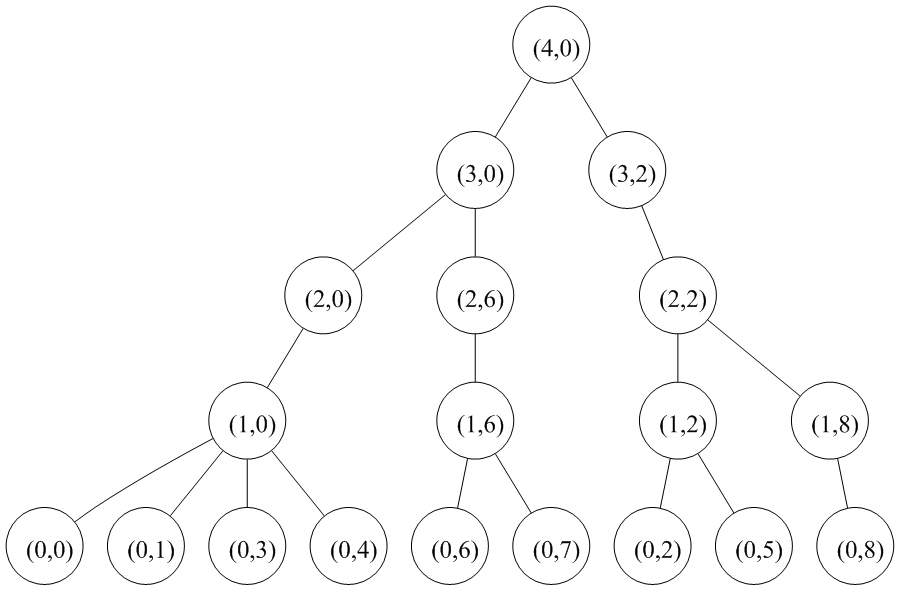
\includegraphics[width=.45\linewidth]{ipfs-forest-unzipping-a-hierarchy.png}}%
	\hspace{8mm}%
	\subfigure[After splitting $(1,2)$]{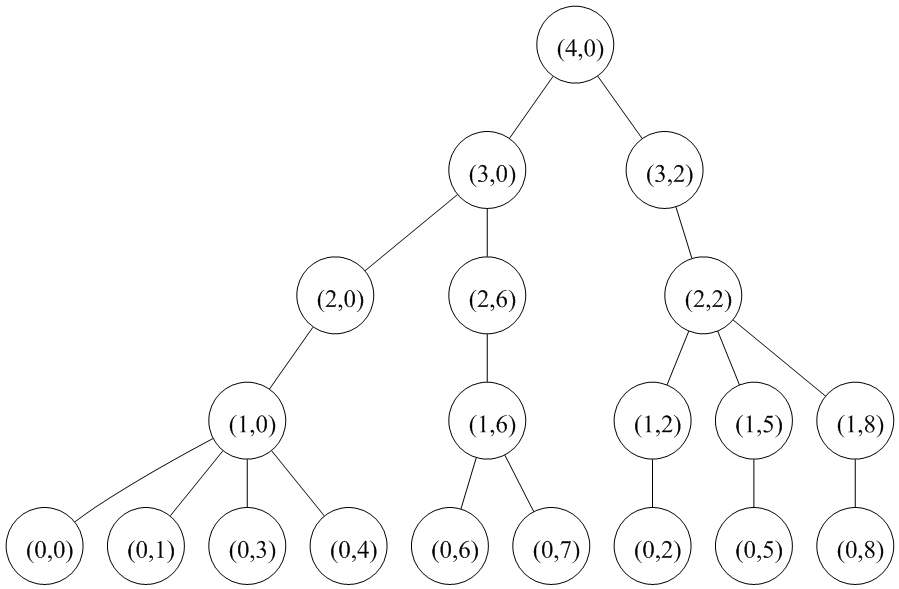
\includegraphics[width=.45\linewidth]{ipfs-forest-unzipping-b-hierarchy.png}}%
	\\
	\subfigure[After splitting $(2,2)$]{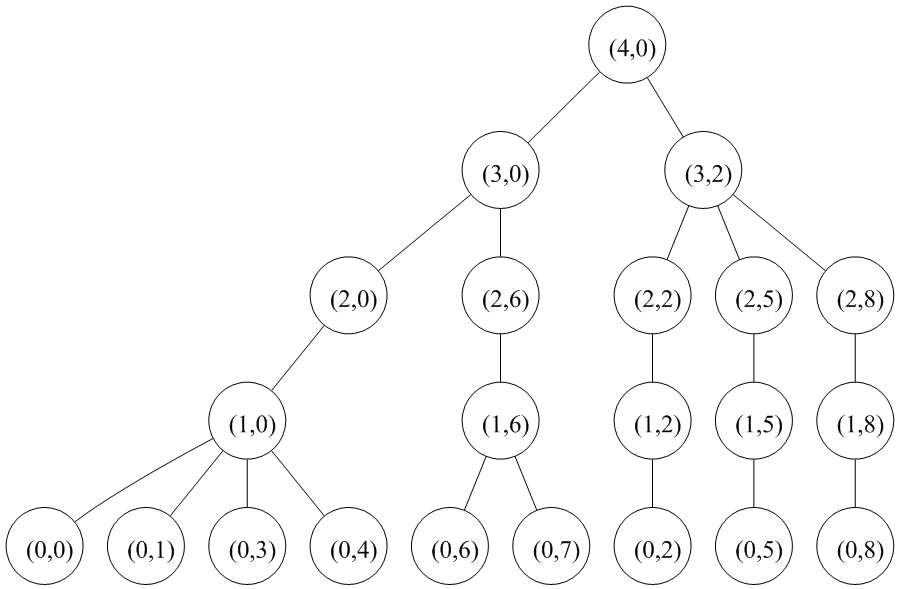
\includegraphics[width=.45\linewidth]{ipfs-forest-unzipping-c-hierarchy.png}}%
	\hspace{8mm}%
	\subfigure[After splitting $(3,2)$]{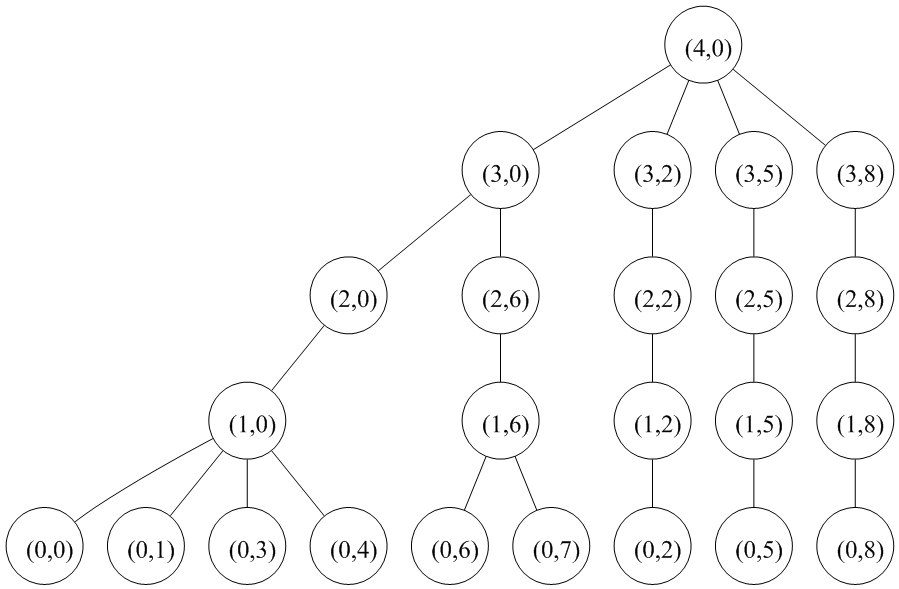
\includegraphics[width=.45\linewidth]{ipfs-forest-unzipping-d-hierarchy.png}}%
	%\\
	%\subfigure[Initial layer $1$ graph]{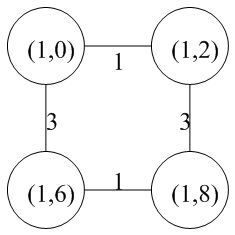
\includegraphics[width=.22\linewidth]{ipfs-forest-unzipping-a-graph1.png}}%
	%\hspace{8mm}%
	%\subfigure[Initial layer $2$ graph]{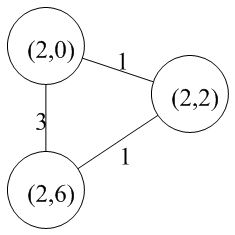
\includegraphics[width=.22\linewidth]{ipfs-forest-unzipping-a-graph2.png}}%
	%\hspace{8mm}%
	%\subfigure[Initial layer $3$ graph]{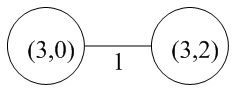
\includegraphics[width=.22\linewidth]{ipfs-forest-unzipping-a-graph3.png}}%
	%\\
	%\subfigure[Final layer $1$ graph]{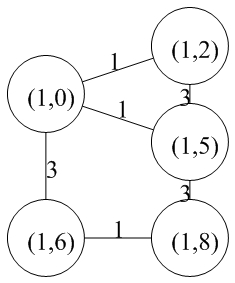
\includegraphics[width=.22\linewidth]{ipfs-forest-unzipping-b-graph1.png}}%
	%\hspace{8mm}%
	%\subfigure[Final layer $2$ graph]{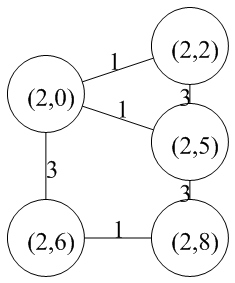
\includegraphics[width=.22\linewidth]{ipfs-forest-unzipping-c-graph2.png}}%
	%\hspace{8mm}%
	%\subfigure[Final layer $3$ graph]{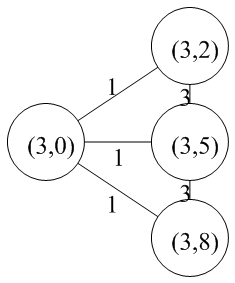
\includegraphics[width=.22\linewidth]{ipfs-forest-unzipping-d-graph3.png}}%
\caption{An example of unzipping: unzipping node $(0,5)$ to layer $3$}
\label{fig:ipfs-forest-unzipping}
\end{stusubfig}
%---

\subsection{Zip Chains}

%---
\begin{stulisting}[t]
\caption{Zip Chains: Implementation}
\label{code:ipfs-forest-zipchains}
\lstinputlisting[style=Default]{ipfs-forest-zipchains.lst}
\end{stulisting}
%---

A set of node chains that all start in the same layer can be zipped together, an operation that is effectively a multi-layer sibling node merge. Zipping takes as input $k$ chains $[n_{1h},...,n_{1\ell_1}],...,[n_{kh},...,n_{k\ell_k}]$ and returns the node and layer index that would be needed by an unzip to undo the operation. See Figure~\ref{fig:ipfs-forest-zipping} for an example.

The implementation of zipping is straightforward (see Listing~\ref{code:ipfs-forest-zipchains}), but there are a number of important preconditions that must be checked before the main operation in order to avoid invalid zips:
%
\begin{enumerate}
\item There must be chains to zip.
\item Each chain must be non-empty and consist only of valid nodes.
\item No chain must extend down as far as the leaf layer of the forest -- this prevents the merging of leaf layer nodes.
\item The highest nodes in the chains must be siblings of each other.
\item The sets of nodes to be merged in each layer must be connected.
\end{enumerate}
%
For valid zips, we start by determining the high and low layers of the chains. All the chains share the same high layer, so it suffices to take the high layer of the first chain in the array. The low layer is determined by a simple minimum element operation on the low layers of each of the individual chains. For each of the layers, from the top down, the relevant nodes are then extracted from the chains and merged using sibling node merging.

%---
\begin{stusubfig}{p}
	\subfigure[Initial hierarchy]{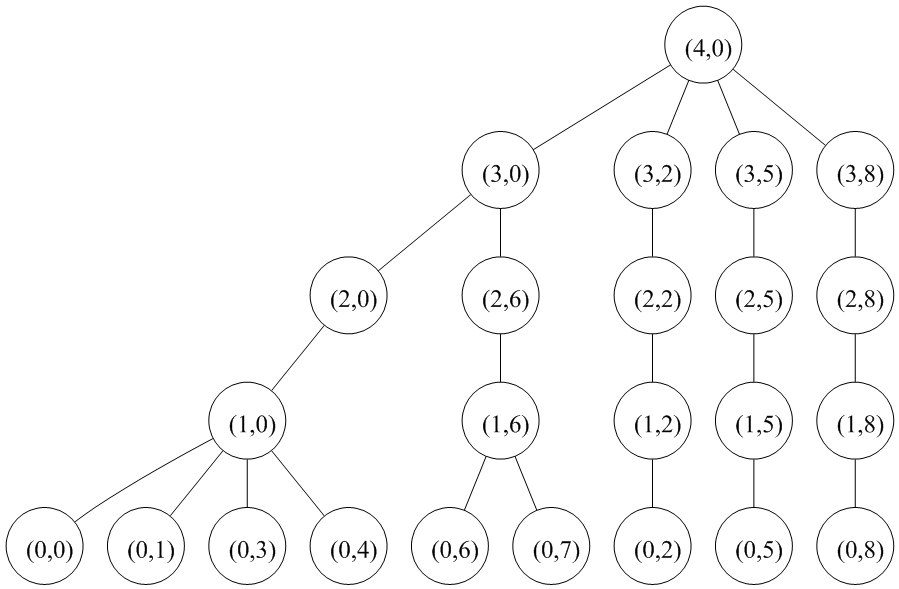
\includegraphics[width=.43\linewidth]{ipfs-forest-zipping-a-hierarchy.png}}%
	\hspace{8mm}%
	\subfigure[After merging layer $3$ nodes]{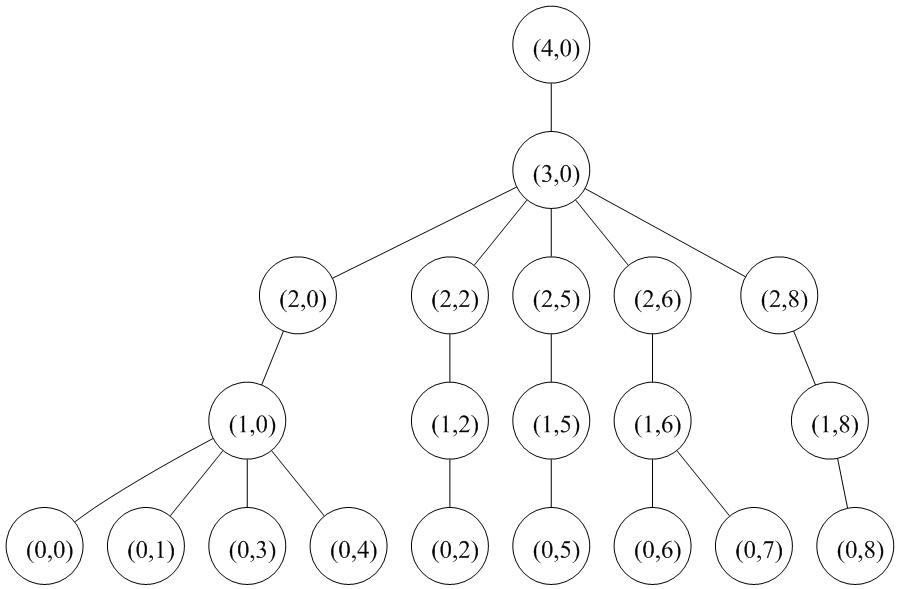
\includegraphics[width=.43\linewidth]{ipfs-forest-zipping-b-hierarchy.png}}%
	\\
	\subfigure[After merging layer $2$ nodes]{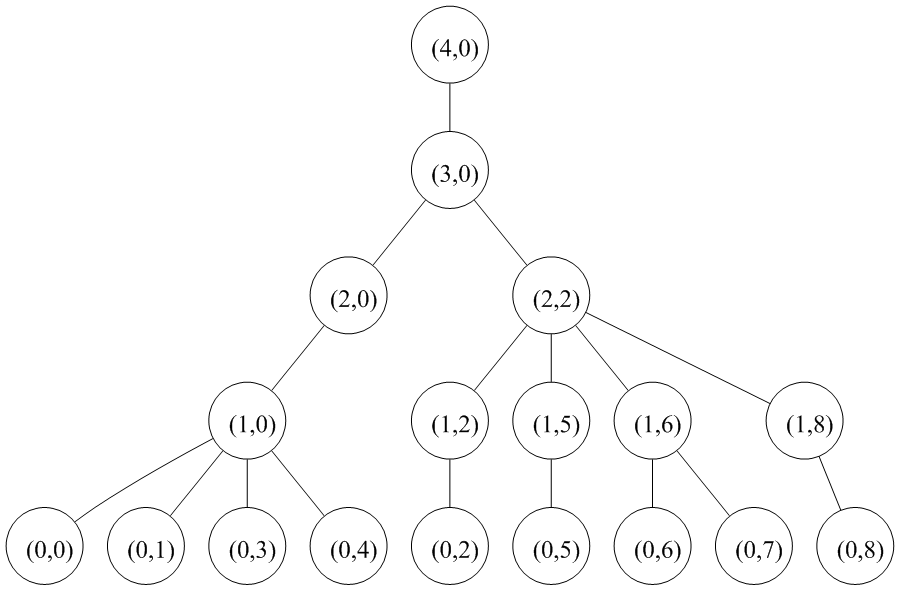
\includegraphics[width=.43\linewidth]{ipfs-forest-zipping-c-hierarchy.png}}%
	\hspace{8mm}%
	\subfigure[After merging layer $1$ nodes]{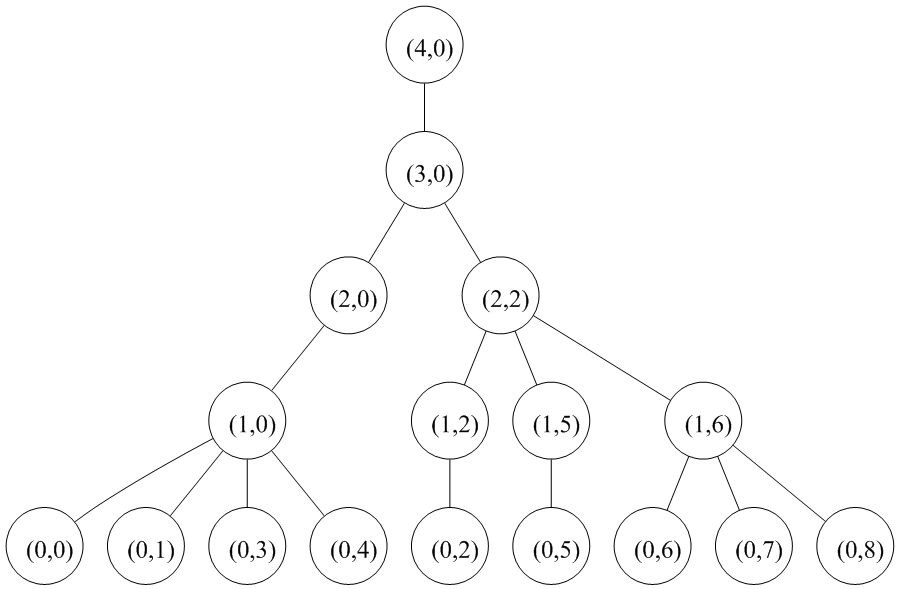
\includegraphics[width=.43\linewidth]{ipfs-forest-zipping-d-hierarchy.png}}%
	%\\
	%\subfigure[Initial layer $1$ graph]{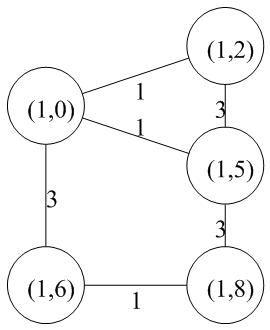
\includegraphics[width=.22\linewidth]{ipfs-forest-zipping-a-graph1.png}}%
	%\hspace{8mm}%
	%\subfigure[Initial layer $2$ graph]{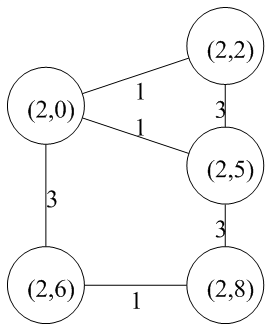
\includegraphics[width=.22\linewidth]{ipfs-forest-zipping-a-graph2.png}}%
	%\hspace{8mm}%
	%\subfigure[Initial layer $3$ graph]{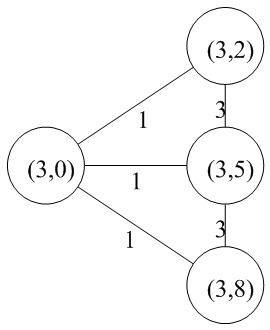
\includegraphics[width=.22\linewidth]{ipfs-forest-zipping-a-graph3.png}}%
	%\\
	%\subfigure[Final layer $1$ graph]{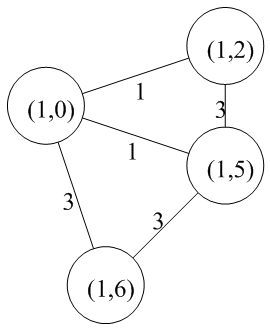
\includegraphics[width=.22\linewidth]{ipfs-forest-zipping-d-graph1.png}}%
	%\hspace{8mm}%
	%\subfigure[Final layer $2$ graph]{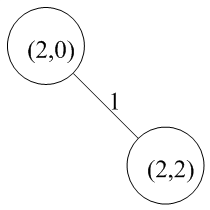
\includegraphics[width=.22\linewidth]{ipfs-forest-zipping-c-graph2.png}}%
	%\hspace{8mm}%
	%\subfigure[Final layer $3$ graph]{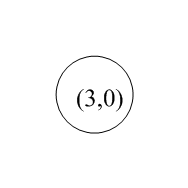
\includegraphics[width=.22\linewidth]{ipfs-forest-zipping-b-graph3.png}}%
\caption{An example of zipping: zipping together the four chains $[(3,0), (2,6), (1,6)]$, $[(3,2), (2,2)]$, $[(3,5), (2,5)]$ and $[(3,8), (2,8), (1,8)]$}
\label{fig:ipfs-forest-zipping}
\end{stusubfig}
%---

%#################################
\section{Non-Sibling Node Merging}
\label{sec:nsmerge}
%#################################

%---
\begin{stulisting}[t]
\caption{Non-Sibling Node Merging: Implementation}
\label{code:ipfs-forest-mergenonsiblingnodes}
\lstinputlisting[style=Default]{ipfs-forest-mergenonsiblingnodes.lst}
\end{stulisting}
%---

Having discussed unzipping and zipping, we are now in a position to implement the non-sibling node merging operation mentioned previously: this allows the user to merge nodes based on their adjacency in the image rather than on whether or not they share a common parent in the IPF. This is the `intuitive' merge operation that users might want to perform, but it is difficult to implement without the machinery provided by the zipping algorithms.

Non-sibling node merging involves taking a set of arbitrary nodes in any layer of the hierarchy other than the lowest, dividing it into its connected components and then merging the nodes in each one individually (using a combination of unzipping and zipping). Since each component is connected, the result of each merge represents a contiguous image region. The algorithm takes as input the set of nodes to be merged, and returns the set of nodes resulting from merging each of the input's connected components (i.e.~there is one output node for each connected component of the input). See Figure~\ref{fig:ipfs-forest-nonsiblingnodemerging} for an example.

The implementation is shown in Listing~\ref{code:ipfs-forest-mergenonsiblingnodes}. The first step is to calculate the connected components of the input nodes: each connected component of size $> 1$ will be merged into one result node. To perform the merge for each connected component, we first determine the common ancestor of the component's nodes. Each node is then unzipped to the layer below that containing the ancestor. In each case we keep track of the chain of nodes leading back down to the node being unzipped, appending the actual node being unzipped to the chain in each case (it would not otherwise be present). Finally, all of these chains are zipped together to merge the nodes in the connected component together.

For the example in Figure~\ref{fig:ipfs-forest-nonsiblingnodemerging}, the connected components of the input nodes are $\{(1,0),(1,2)\}$ and $\{(1,6),(1,8)\}$. Both $(1,0)$ and $(1,2)$ are unzipped to layer $2$, the layer below their common ancestor $(3,0)$. The chains thus created are then zipped together, resulting in $(1,0)$ and $(1,2)$ being merged in layer $1$. An analogous process is used to merge $(1,6)$ and $(1,8)$.

%---
\begin{stusubfig}{p}
	\subfigure[Initial hierarchy]{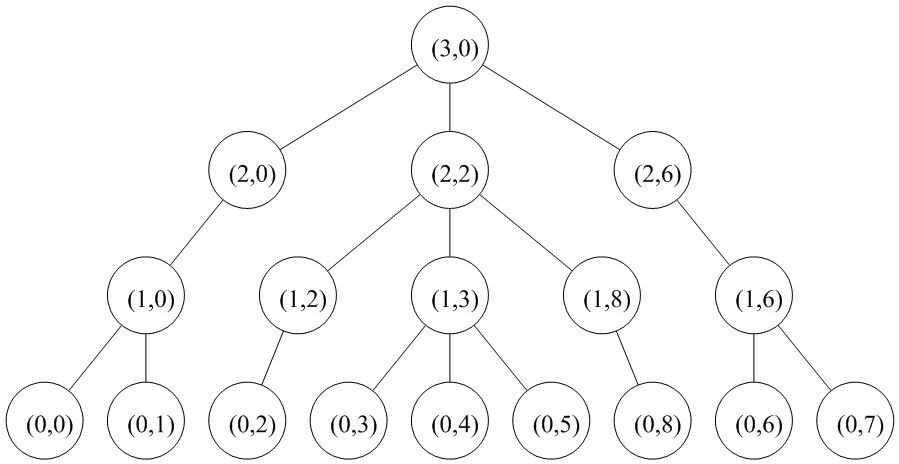
\includegraphics[width=.45\linewidth]{ipfs-forest-nonsiblingnodemerging-a-hierarchy.png}}%
	\hspace{8mm}%
	\subfigure[After unzipping $(1,0)$ and $(1,2)$ to layer $2$]{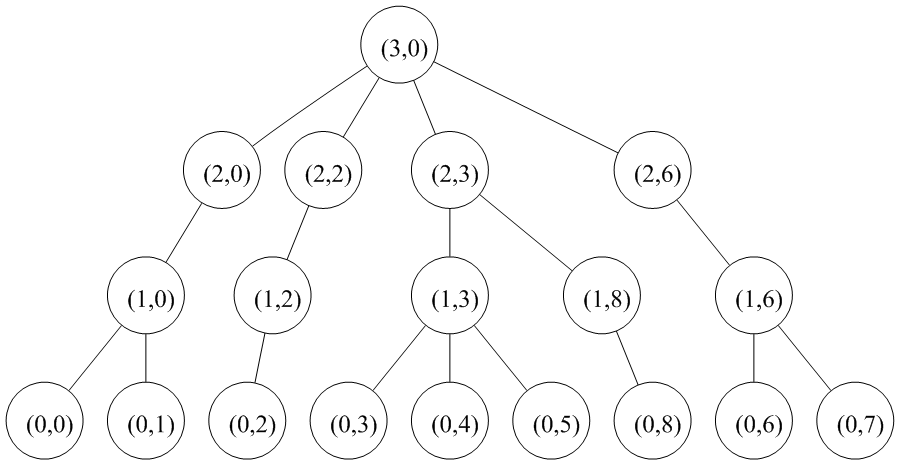
\includegraphics[width=.45\linewidth]{ipfs-forest-nonsiblingnodemerging-c-hierarchy.png}}%
	\\
	\subfigure[{After zipping $[(2,0), (1,0)]$ and $[(2,2), (1,2)]$}]{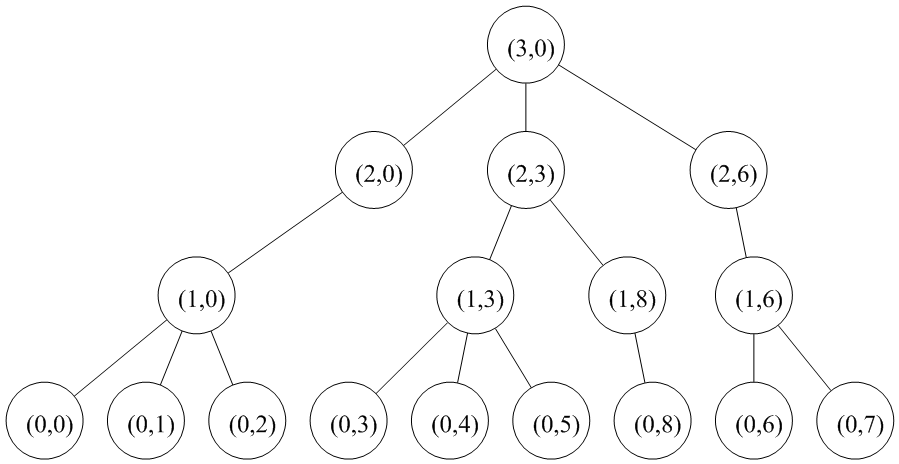
\includegraphics[width=.45\linewidth]{ipfs-forest-nonsiblingnodemerging-d-hierarchy.png}}%
	\hspace{8mm}%
	\subfigure[After unzipping $(1,6)$ and $(1,8)$ to layer $2$]{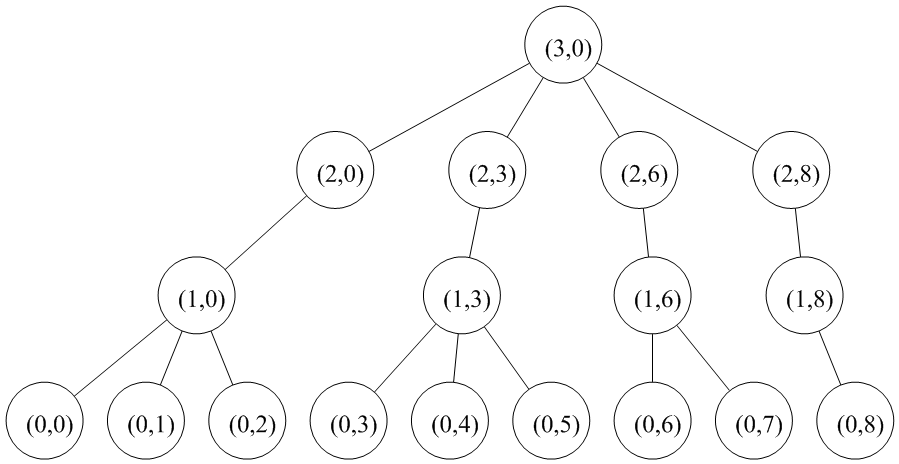
\includegraphics[width=.45\linewidth]{ipfs-forest-nonsiblingnodemerging-f-hierarchy.png}}%
	\\
	\subfigure[{After zipping $[(2,6), (1,6)]$ and $[(2,8), (1,8)]$}]{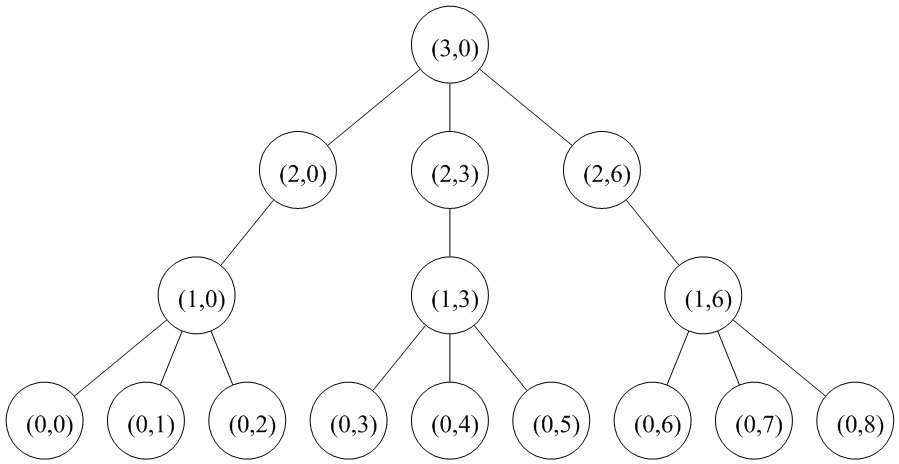
\includegraphics[width=.45\linewidth]{ipfs-forest-nonsiblingnodemerging-g-hierarchy.png}}%
\caption{An example of non-sibling node merging: merging nodes $(1,0)$, $(1,2)$, $(1,6)$ and $(1,8)$}
\label{fig:ipfs-forest-nonsiblingnodemerging}
\end{stusubfig}
%---

%#########################
\section{User Interaction}
\label{sec:ui}
%#########################

In this section, we illustrate the practicality of the algorithms in this paper by presenting a concrete implementation of them in \emph{millipede}, a cross-platform tool for 3D segmentation, feature identification and visualisation. We also evaluate the benefits of the non-sibling node merging algorithm from the user's perspective, demonstrating in particular that non-sibling node merging (a) is needed for a significant proportion of the potential merges that a user might want to perform, and (b) considerably reduces the interactivity burden on the user for individual merges.

\subsection{Concrete Implementation}

TODO

\subsection{Evaluation}
\label{subsec:ui-evaluation}

%---
\stufigexx{width=.6\linewidth}{pairwisenodemerges.png}{The percentages of pairwise merges of nodes in various IPFs (all with $5$ branch layers) that require different levels of unzipping (see \S\ref{subsec:ui-evaluation}).}{fig:pairwisenodemerges}{p}
%---

In order to demonstrate the need for non-sibling node merging and its effectiveness, we modified the \emph{millipede} software to calculate the number of levels of unzipping that would be required to merge each adjacent pair of nodes in an IPF. (Nodes with the same parent require no unzipping, and can thus be merged by the sibling node merge algorithm; nodes whose parents differ must be unzipped up to their common ancestor as part of a non-sibling node merge.) We calculated how many levels of unzipping were required for all adjacent node pairs in the IPFs of three 3D image datasets (BT, MC and SD) of size $512 \times 512 \times 11$ (see Figure~\ref{fig:pairwisenodemerges}). Each IPF contained $5$ branch layers in addition to its leaf layer. We make the following observations:
%
\begin{itemize}
\item For each IPF, there was a high cumulative percentage ($> 70\%$) of node pairs that required at least one level of unzipping to merge (i.e~that involved \emph{non-sibling} node merging). There was also a relatively high cumulative percentage ($\approx 50\%$) of node pairs that required at least two levels of unzipping to merge. As such, not only do the majority of the potential merges the user might want to perform involve non-sibling node merging, they often involve changes that require multiple levels of unzipping. This is costly in a number of different ways: each individual node split that is required as part of the unzip operation has relatively high input requirements (recall the need to specify the split components), there are corresponding sibling node merges to be performed, and keeping track of the changes required to the IPF without an easy way to visualise the parent-child links carries a high cognitive overhead. Whilst we could circumvent this problem by simply restricting the user to sibling-only node merging, this would prohibit many useful merges. This motivates the development of a non-sibling node merging algorithm of the kind described in this paper: with such an algorithm available, each pairwise node merge becomes a simple operation in the UI (select the two nodes and click to merge).

\item In reality, many node merges are not pairwise -- the user often wants to combine many regions of the image at once. In this case, there is an even higher probability that multiple levels of unzipping will be required.
\end{itemize}
%

%######################
\section{Conclusions}
\label{sec:conclusions}
%######################

Despite the ubiquitous nature of IPFs in the literature, comparatively
little research appears to have been done in the past into ways of
conveniently editing one after it has been constructed.

We have fixed this 

These are basic algorithms but have immediate applications

Zipping and unzipping are instrumental to other segmentation--related
algorithms, such as raising a region to a higer layer, etc.

This has been a description of an abstract data type, but of course
the applications are unlimited in scope and wonderful.

TODO

\clearpage

\bibliographystyle{alpha}
\bibliography{existingwork,mypapers}

\begin{IEEEbiography}[{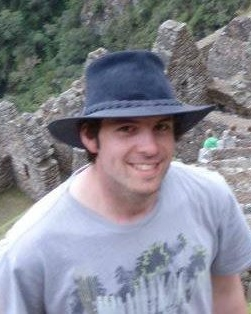
\includegraphics[width=1in,height=1.25in,clip,keepaspectratio]{pic_stuart.jpg}}]{Stuart Golodetz}
Stuart Golodetz obtained his DPhil in Computer Science at Oxford University, working on 3D image segmentation and feature identification. He then spent two interesting years in industry, working in the areas of credit risk management, logic programming and software analytics. His areas of interest include medical image analysis, computer games development and the intricacies of different programming languages, especially C++. He was a session chair for the 6th International Symposium on Image and Signal Processing and Analysis, ISPA 2009. He is a member of the Association of C and C++ Users (ACCU) and has written a number of articles for their magazines.
\end{IEEEbiography}

\begin{IEEEbiography}[{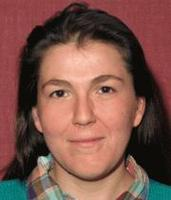
\includegraphics[width=1in,height=1.25in,clip,keepaspectratio]{pic_irina.jpg}}]{Irina Voiculescu}
TODO
\end{IEEEbiography}

\begin{IEEEbiography}[{
\includegraphics[width=1in,height=1.25in,clip,keepaspectratio]{pic_stephen.jpg}}]{Stephen Cameron}
Stephen Cameron obtained his PhD in Artificial Intelligence at Edinburgh University, working on the geometric modelling of robots and on collision detection. His general area of interest is in spatial reasoning, although this covers a wide range which includes the planning of tasks and motions for robot vehicles and manipulators, the use of geometric models, and the scheduling of fleets of robots. Some of his work is in collaboration with members of the Oxford University Robotics Research Group in the Department of Engineering Science. He is a member of the AISB, the IEEE Robotics and Automation Society, the Geometric Modelling Society, the IAM and CAMRA.
\end{IEEEbiography}

\end{document}
